\chapter{Analysis and Design}

\section{ROS and YuMi Overview}
As discussed in the Background Chapter, ROS handles a number of independent Nodes that performs specific function(s). They communicate with each other by publishing messages to topics or subscribing them. ROS messages support several data formats, including number, string, and time etc. Moreover, these communications are only available if a $roscore$ is running, which is a collection of programs and Nodes that are prerequisites of a ROS-based system.

Besides, $TF$ is an important package in ROS and used several times in this project. According to \citep{tfROSWik}, it maintains the relationship between coordinate frames (such as camera frame, robot fram etc.) in a tree structure buffered, which enables the user to transform points, vectors, etc between any two coordinate frames at any desired point in time. Details will be discussed in Implementation Chapters.

The dual-arm robot YuMi communicates with ROS using Personal Robotics Lab setup (User Guide Chapter contains more details). YuMi has one gripper camera embedded in each of its gripper. Using these cameras may provide more accurate results of shoe and shoe hole locations. However, in order to use these two cameras, a package named $abb\_rws\_interface$ which is a proprietary interface of ABB is required. According to \citep{EGMfiles}, it is not public. Also, the open source version of that package called $abb\_librws$ cannot match the current $yumi\_cameras$ setup. Furthermore, it is not very feasible to tie a small camera to YuMi's arms. Therefore, this project will only utilize the ASUS Xtion or ZED Mini camera for detection.

\section{System Overview}

\begin{figure}[H]
\centering
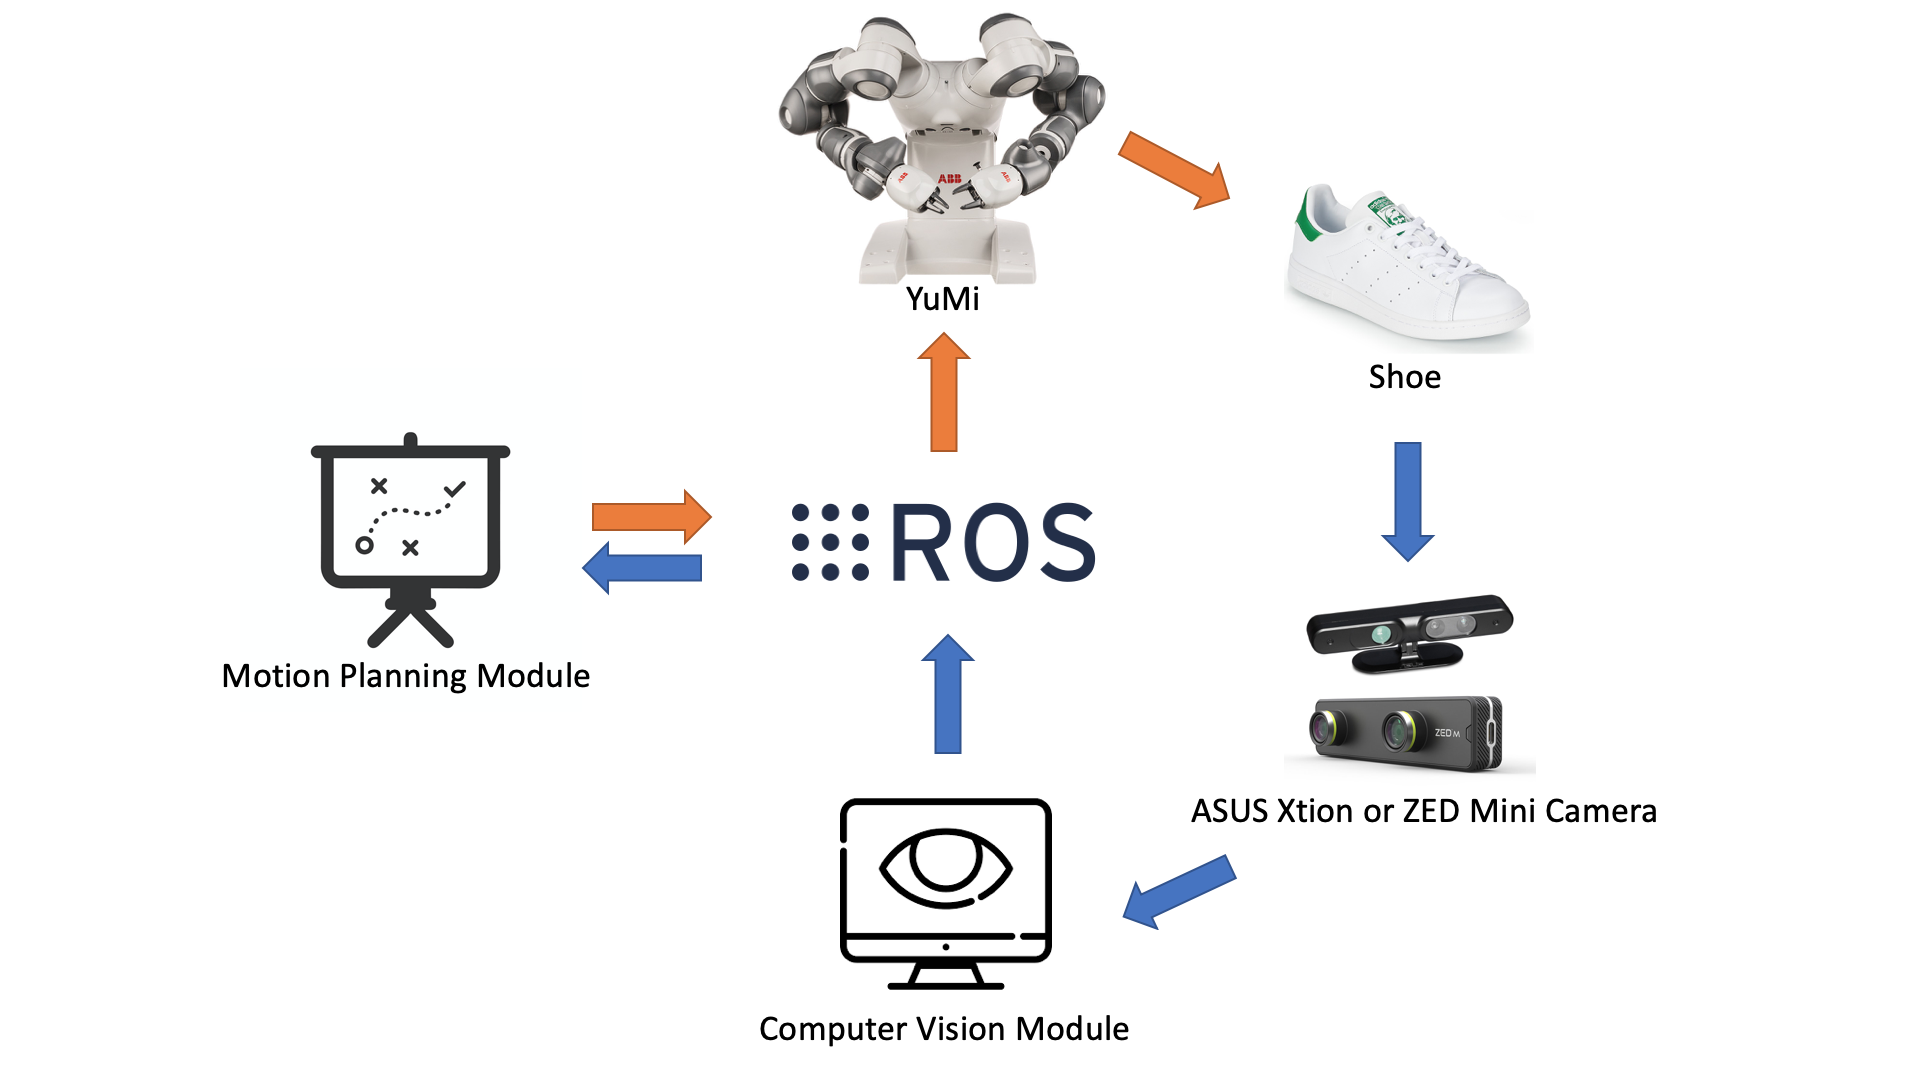
\includegraphics[width = \columnwidth]{AnalysisDesign/system.png}
\caption{System overview}
\label{c4}
\end{figure}

Figure \ref{c4} displays the system overview of this project, which consists six components: the shoe, the camera, computer vision module, ROS Kinetic, motion planning module, and YuMi. Blue arrows represent computer vision messages and orange arrows indicate related motion plans and manipulations.

Starting from the camera, which consistently recording RGB and depth images of the workbench and outputs them to the computer vision module. The module then performs several functions including shoe detection, shoe hole tracking, 6D shoe hole pose estimation etc and publishes the corresponding message to ROS topics. After that, the motion planning module subscribes these information and plans YuMi arms trajectories accordingly to adjust shoe pose or put lace on a hole. If the planning succeeds, YuMi will then execute these motions to manipulate shoe and shoe lace.

%detail---------------------------
\section{System Workflow}

\begin{figure}[H]
\centering
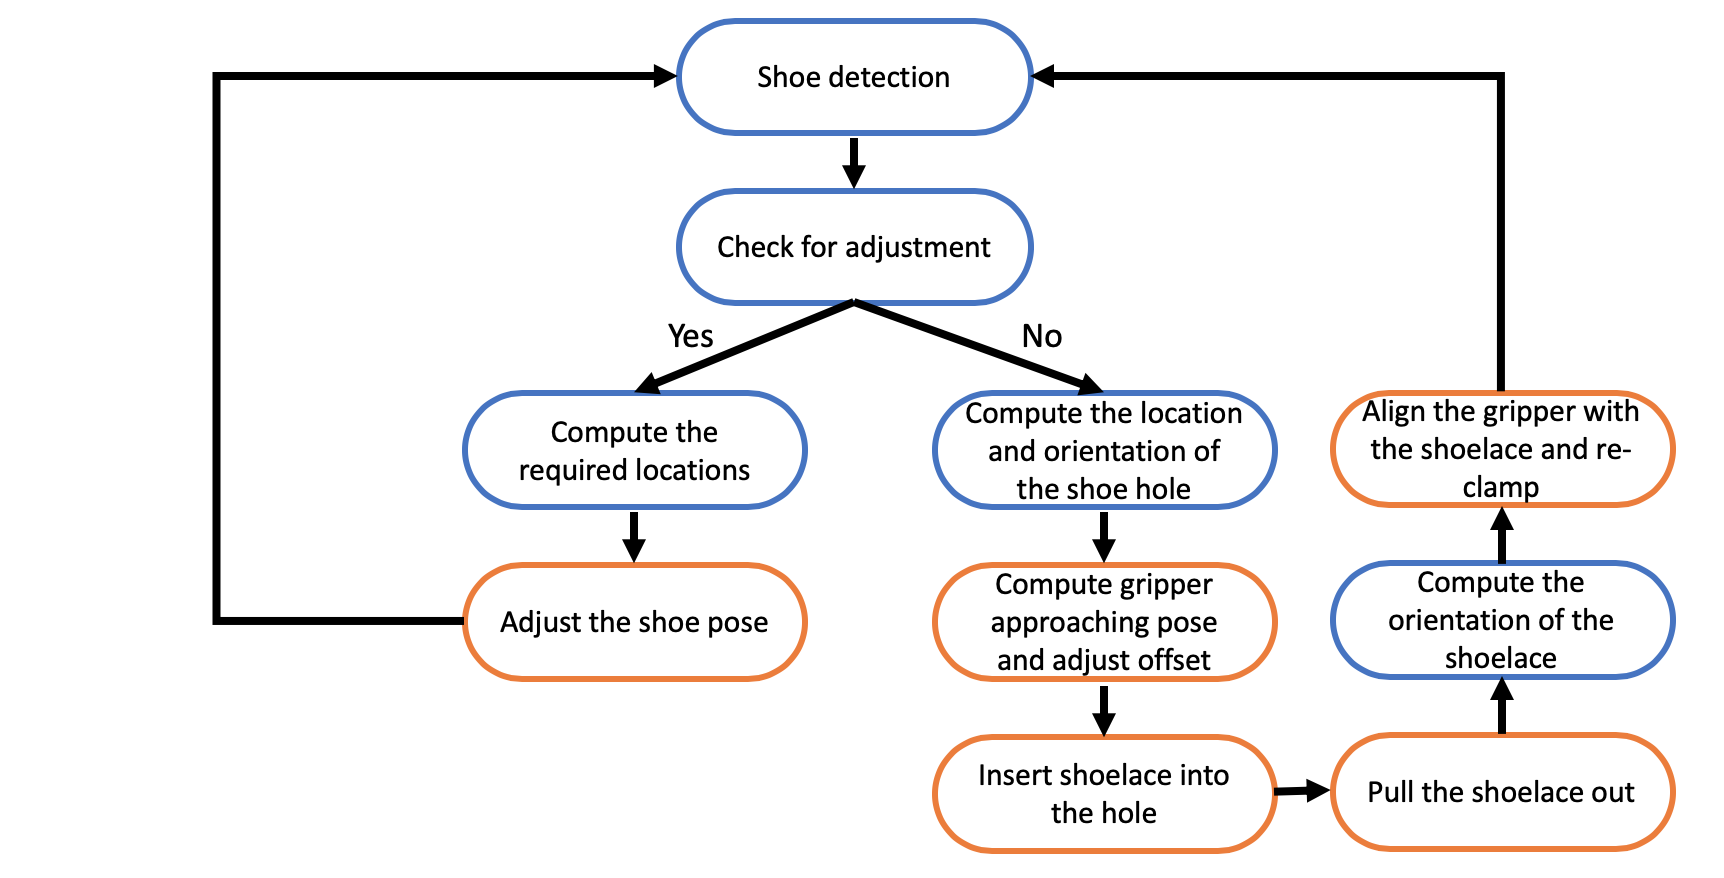
\includegraphics[width = \columnwidth]{AnalysisDesign/workflow.png}
\caption{System workflow}
\label{workflow}
\end{figure}

discussion ................

The following two chapters will discuss detailed implementation approaches.